\subsubsection{アーキテクチャビューとビューポイント}
\keyterm{ビュー}\en{architecture view}とは、アーキテクチャの一面を表すものである。たとえば、機能要求をどう満たすかを示す論理ビュー、並行処理や実行時相互作用を示すプロセスビュー、システムをどこに配置するかを示す物理ビュー、実装単位や依存関係を示す開発ビューがある。

ビューを分ける理由は、関心事を分離するためである。性能を確認したい人、安全性を確認したい人、配置を考える人、コード分担を考える人は、それぞれ必要な情報が違う。一つの図にすべてを詰め込むと、誰にとっても読みにくい図になる。

\keyterm{ビューポイント}\en{architecture viewpoint}とは、ビューを作成し、解釈し、利用するための規約である。どの要素を使うか、どの関係を描くか、どの記法を使うか、どの関心事に答えるか、誰が読むかを定める。ビューポイントは、ビューの「描き方の型」である。

\par\smallskip\noindent\refstepcounter{table}\label{tab:ch02-03}\textbf{表 \thetable: 第02章 ソフトウェアアーキテクチャ 表03}\par\smallskip
\begin{longtable}{P{0.25\linewidth}P{0.67\linewidth}}
\toprule
種類 & 説明 \\
\midrule
モジュールビューポイント & 実装単位としてのモジュール、その責任、依存関係、分割を表す。 \\
構成要素・接続子ビューポイント & 実行時の大きな構成要素と、それらをつなぐ通信・接続関係を表す。 \\
論理ビューポイント & 対象領域の主要概念、能力、関係を表す。 \\
シナリオ・ユースケースビューポイント & 利用者がシステムとどのように相互作用するかを表す。 \\
情報ビューポイント & 重要な情報、データの保管、アクセス、流れを表す。 \\
配置ビューポイント & ソフトウェアをどの実行環境、機器、ネットワークに置くかを表す。 \\
\bottomrule
\end{longtable}

複数のビューを使うと、別の問題が生じる。ビュー同士が矛盾する可能性である。たとえば、開発ビューでは存在する構成要素が配置ビューにはない、または論理ビューの関係が実行時ビューで説明されていない、といった問題である。これを複数ビュー問題という。対策として、ビュー間の対応関係、追跡可能性、整合性規則を明示する必要がある。

ビューを構成する方法には二つの代表的な考え方がある。\keyterm{合成的手法}では、複数のビューを別々に作り、対応規則で統合する。\keyterm{射影的手法}では、一つの統一モデルから複数のビューを取り出す。射影的手法は整合性を保ちやすいが、統一モデルが表せない関心事には弱い。

\begin{figure}[htbp]
\centering
\IfFileExists{assets/generated_figures/ch02/fig-ch02-04.png}{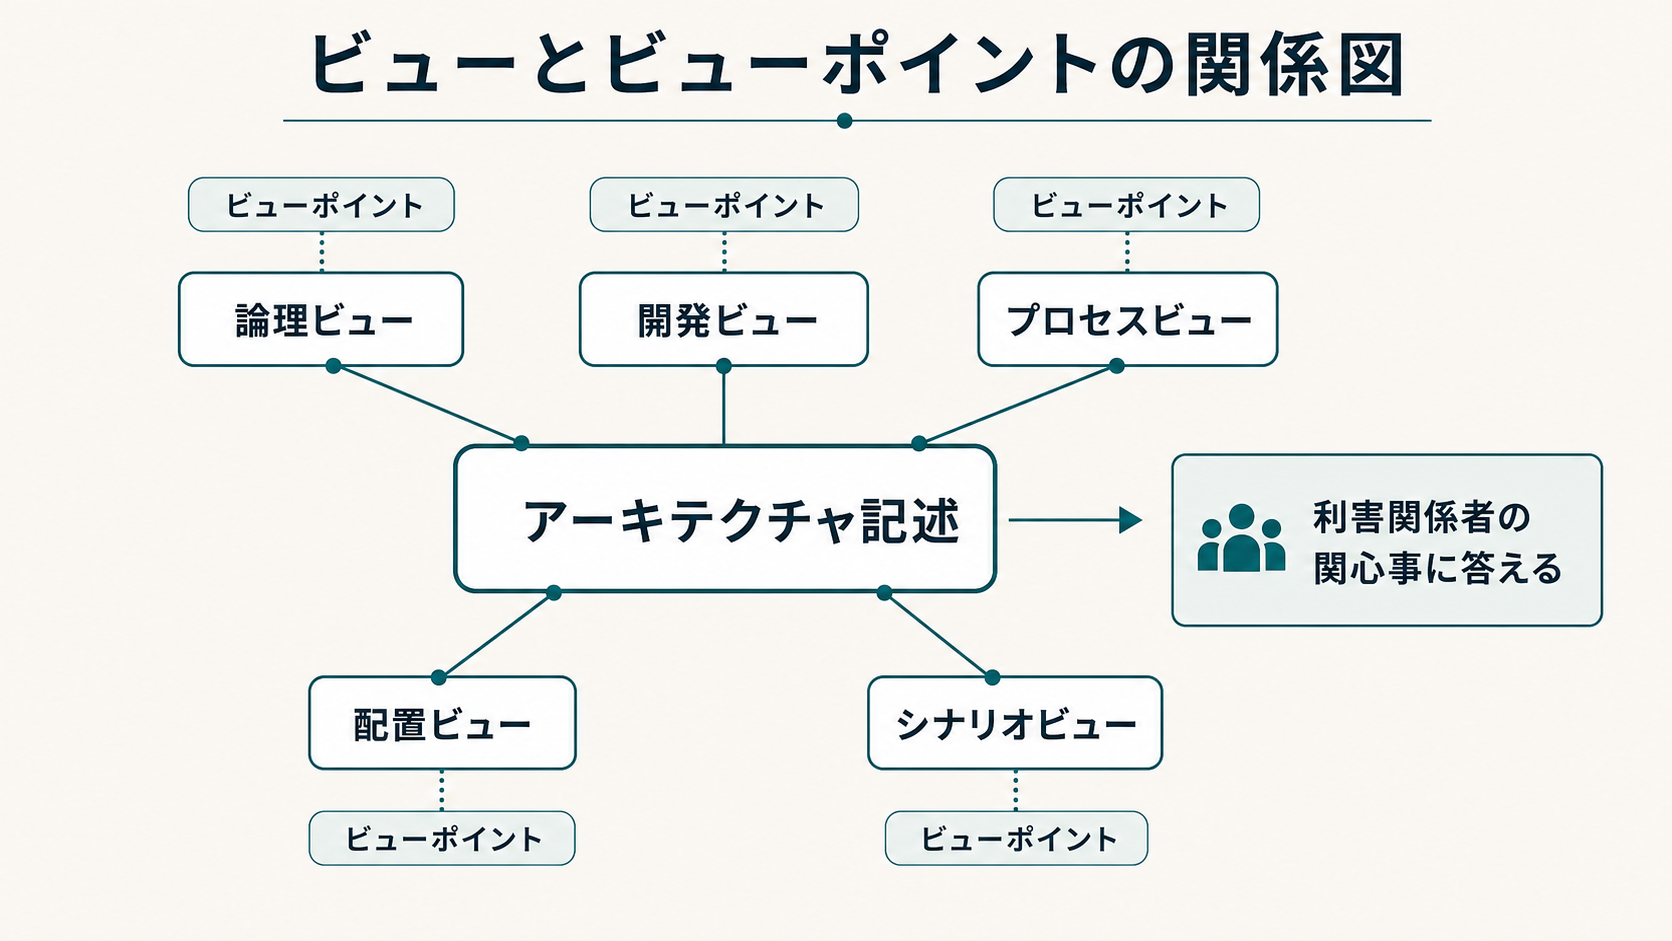
\includegraphics[width=0.96\linewidth]{assets/generated_figures/ch02/fig-ch02-04.png}}{\fbox{\parbox[c][48mm][c]{0.9\linewidth}{\centering 画像生成待ち\\ビューとビューポイントの関係図}}}
\caption{ビューとビューポイントの関係図}
\label{fig:ch02-04}
\end{figure}
